\section{Implementa��o}

\begin{frame}\frametitle{Implementa��o}
\begin{itemize}
	\item OpenSceneGraph para a renderiza��o e carregamento dos modelos.
	\item PQP para a detec��o de colis�o entre as partes.
\end{itemize}
\end{frame}



\begin{frame}\frametitle{Implementa��o}
\begin{itemize}
	\item Vis�o geral:
	\begin{columns}[T]
	\begin{column}{2cm}
	\begin{overprint}
		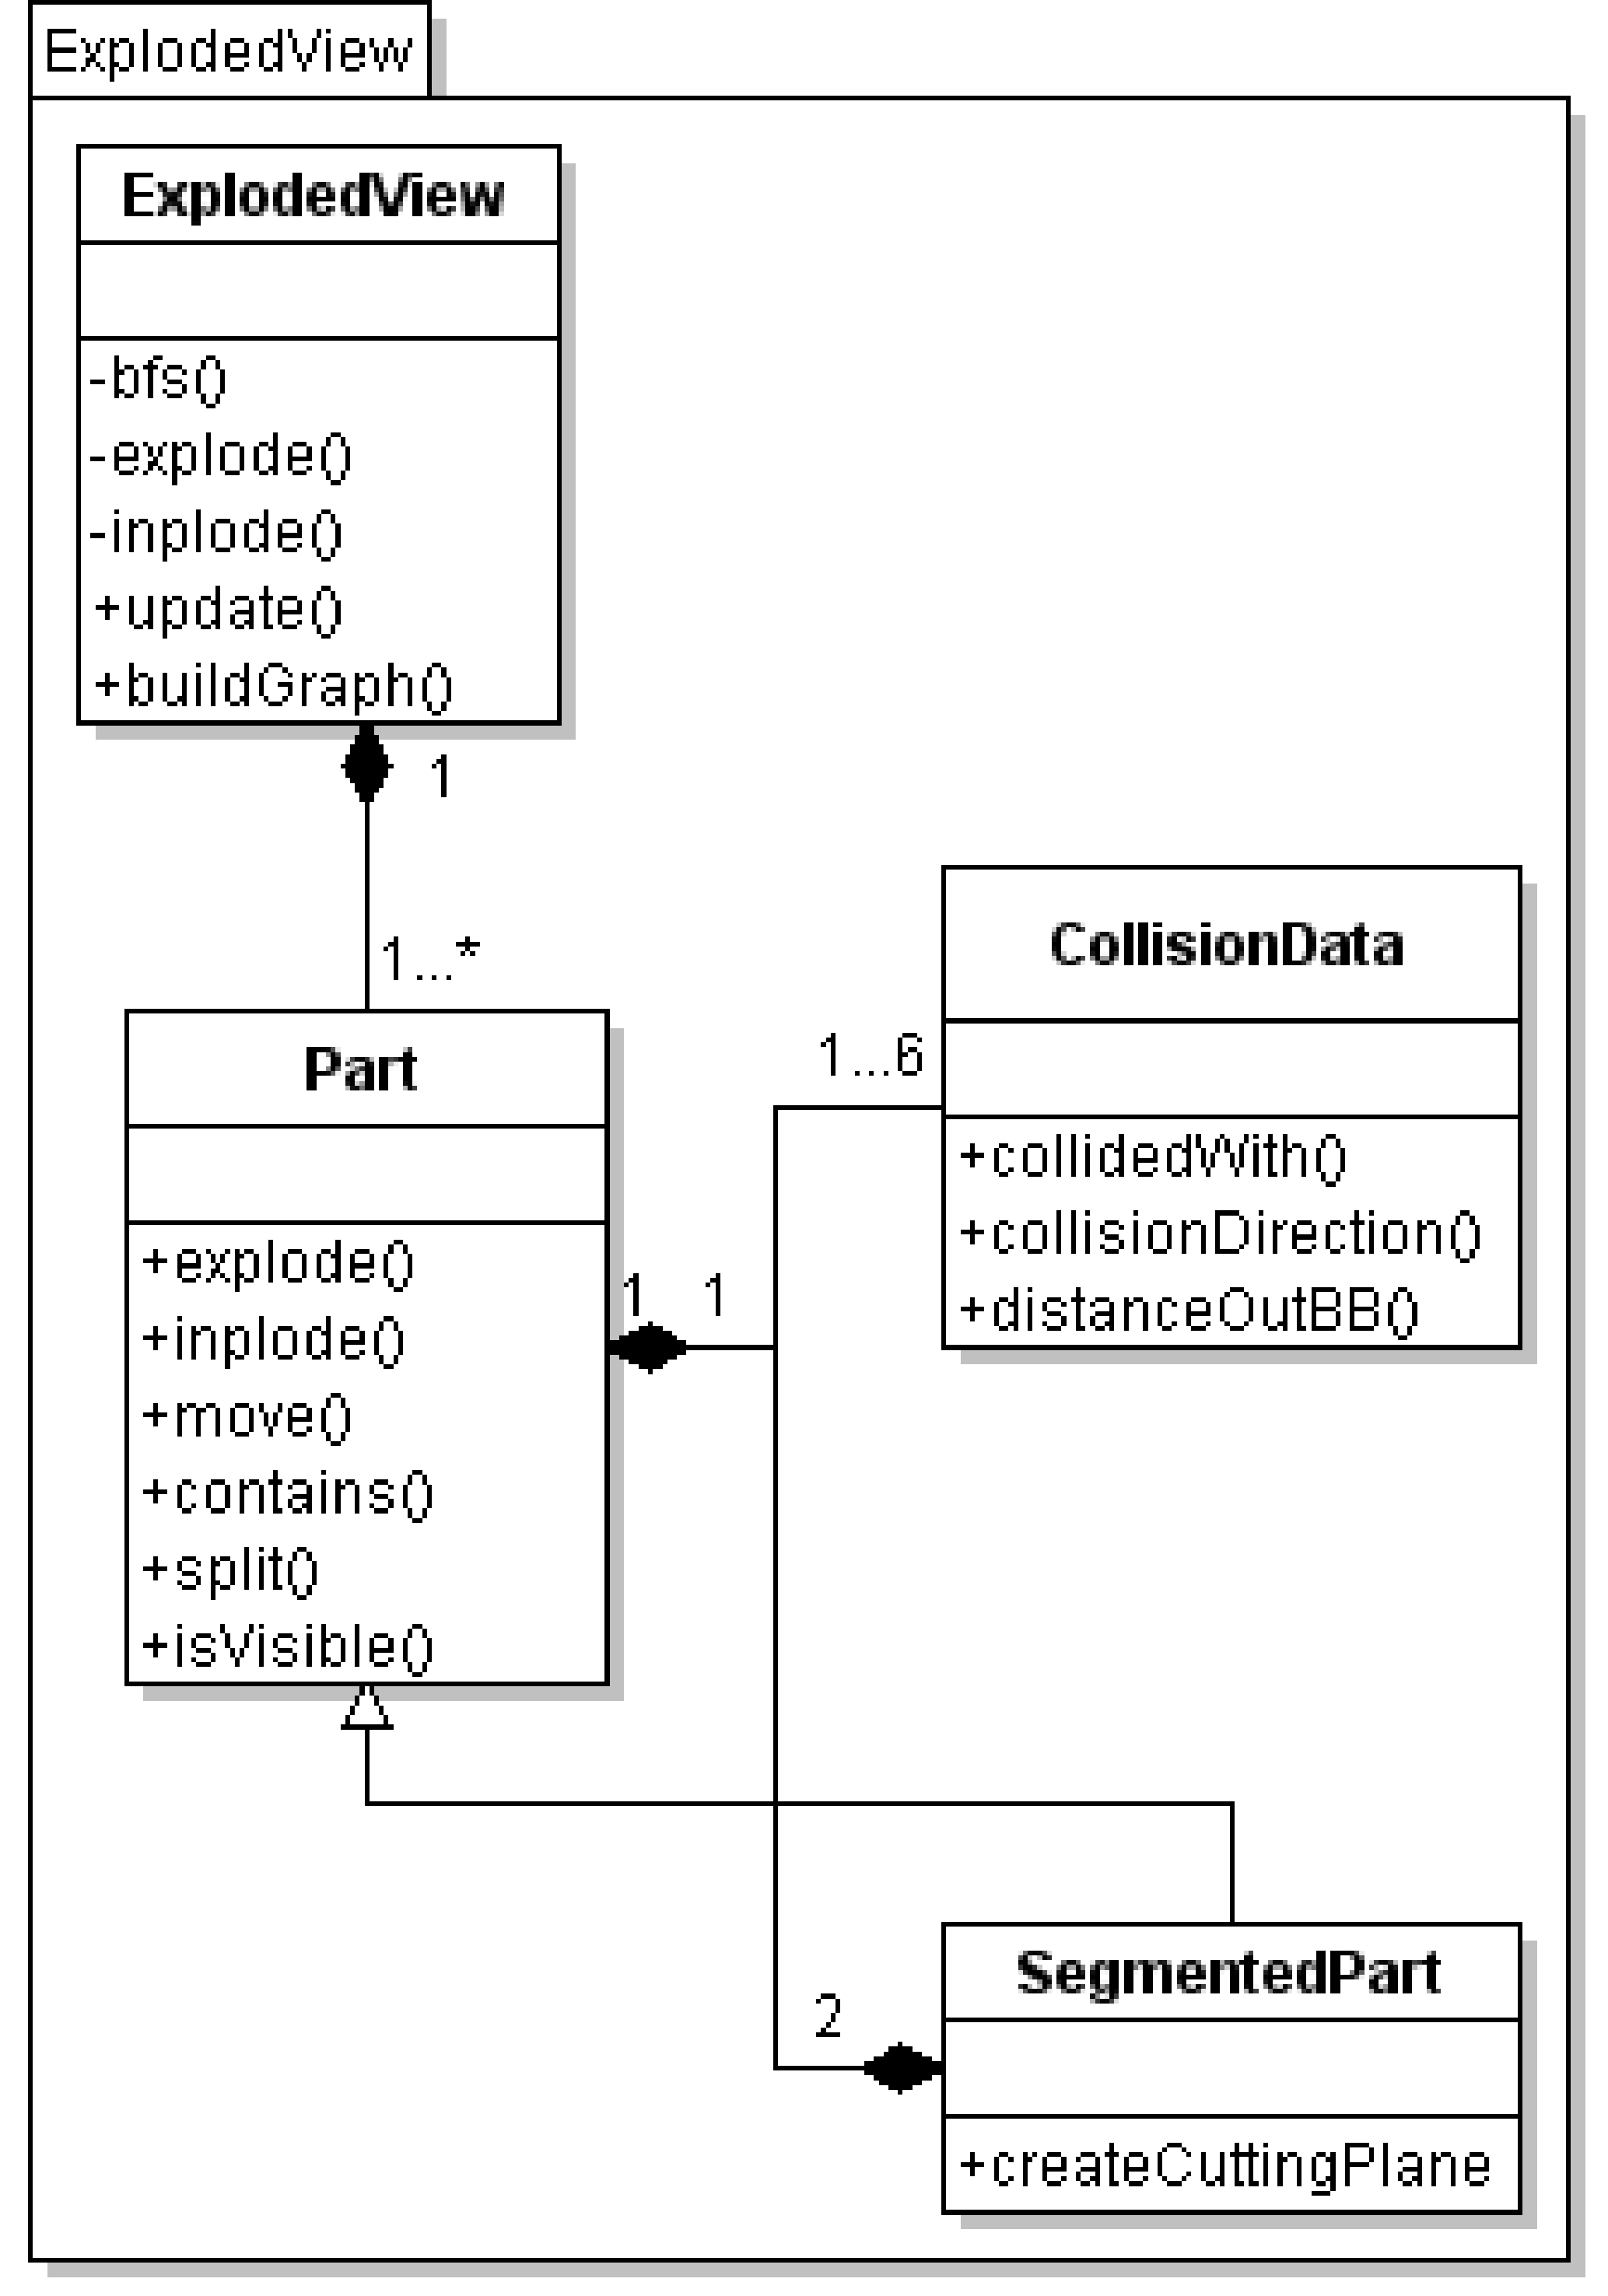
\includegraphics[height=150.0px]{img/arquitetura}
	\end{overprint}
	\vspace{3cm} 
	\end{column}
	\begin{column}{5cm}
	\begin{itemize}
		\item \footnotesize \textbf{ExplodedView}: classe geral, respons�vel pelo por tratar os dados de entrada (tanto o modelo 3D quanto o \emph{input} do usu�rio).
		\item \footnotesize \textbf{Part}: classe que representa as partes do modelo.
		\item \footnotesize \textbf{SegmentedPart}: classe que herda de \textbf{Part} e representa os recipientes divididos. A divis�o dos modelos � feita atrav�s de um \textbf{ClipNode} do \textbf{OSG}.
		\item \footnotesize \textbf{CollisionData}: representa os dados de colis�o.
	\end{itemize}
	\end{column}
	\end{columns}
\end{itemize}
\end{frame}

\begin{frame}\frametitle{Implementa��o}
\center 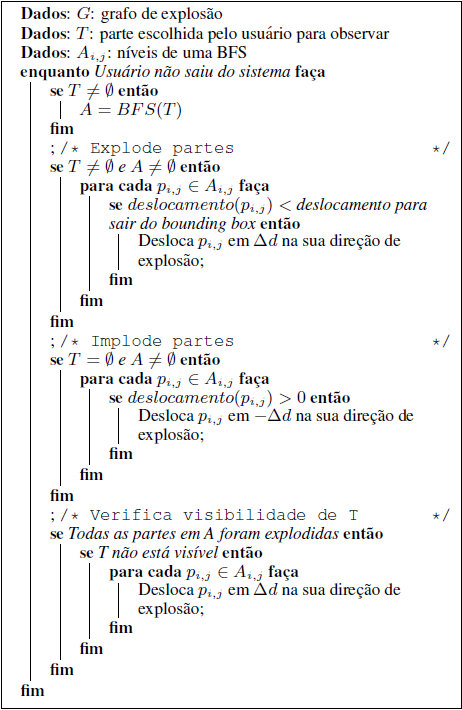
\includegraphics[height=200.0px]{img/algoritmo}
\end{frame}